\documentclass[12pt,a4paper]{article}

% ── Core packages ──────────────────────────────────────────────────────────────
\usepackage[margin=2.5cm]{geometry}
\usepackage[T1]{fontenc}
\usepackage[utf8]{inputenc}
\usepackage{amsmath,amssymb}
\usepackage{xcolor}
\usepackage[most]{tcolorbox}
\usepackage{listings}
\usepackage{tikz}
\usepackage{booktabs}
\usepackage{array}
\usepackage[hidelinks]{hyperref}
\usepackage{float}
\usepackage{caption}
\usepackage{enumitem}
\usepackage{titlesec}
\usepackage{fancyhdr}
\usepackage{algorithm}
\usepackage{algpseudocode}

\usetikzlibrary{arrows.meta, positioning, shapes.geometric, shapes.misc,
                fit, backgrounds, calc, decorations.pathreplacing}

% ── Colours ────────────────────────────────────────────────────────────────────
\definecolor{hdrblue}{RGB}{0,70,140}
\definecolor{boxblue}{RGB}{220,235,255}
\definecolor{boxyellow}{RGB}{255,248,210}
\definecolor{boxgreen}{RGB}{215,245,215}
\definecolor{backcode}{RGB}{246,246,250}
\definecolor{cgreen}{RGB}{0,120,0}
\definecolor{cblue}{RGB}{0,80,200}
\definecolor{cpurple}{RGB}{130,0,200}
\definecolor{cgray}{RGB}{110,110,110}

% ── tcolorbox styles ───────────────────────────────────────────────────────────
\tcbuselibrary{skins,breakable}

\newtcolorbox{formulabox}[1]{
  colback=boxyellow, colframe=orange!75!black,
  fonttitle=\bfseries\small, title=#1, breakable,
  boxrule=0.8pt, arc=4pt
}

\newtcolorbox{definitionbox}[1]{
  colback=boxblue, colframe=hdrblue,
  fonttitle=\bfseries\small, title=#1, breakable,
  boxrule=0.8pt, arc=4pt
}

\newtcolorbox{notebox}{
  colback=boxgreen, colframe=green!55!black,
  fonttitle=\bfseries\small, title=Note,
  breakable, boxrule=0.8pt, arc=4pt
}

% ── Listings (C++) ─────────────────────────────────────────────────────────────
\lstdefinestyle{cpp}{
  language=C++,
  backgroundcolor=\color{backcode},
  commentstyle=\color{cgreen}\itshape,
  keywordstyle=\color{cblue}\bfseries,
  numberstyle=\tiny\color{cgray},
  stringstyle=\color{cpurple},
  basicstyle=\ttfamily\footnotesize,
  breaklines=true, breakatwhitespace=false,
  captionpos=b,
  numbers=left, numbersep=6pt,
  showstringspaces=false, tabsize=2,
  frame=single, framesep=2pt, rulecolor=\color{cgray!40},
  morekeywords={Sophus,SE3d,Eigen,Vector3d,Vector2d,Matrix,ldlt,squaredNorm}
}

\lstdefinestyle{python}{
  language=Python,
  backgroundcolor=\color{backcode},
  commentstyle=\color{cgreen}\itshape,
  keywordstyle=\color{cblue}\bfseries,
  numberstyle=\tiny\color{cgray},
  stringstyle=\color{cpurple},
  basicstyle=\ttfamily\footnotesize,
  breaklines=true, breakatwhitespace=false,
  captionpos=b,
  numbers=left, numbersep=6pt,
  showstringspaces=false, tabsize=4,
  frame=single, framesep=2pt, rulecolor=\color{cgray!40}
}

\lstdefinestyle{json}{
  backgroundcolor=\color{backcode},
  basicstyle=\ttfamily\footnotesize,
  breaklines=true,
  captionpos=b,
  numbers=left, numbersep=6pt,
  frame=single, framesep=2pt, rulecolor=\color{cgray!40},
  morestring=[b]",
  stringstyle=\color{cpurple},
  literate=
    {:}{{{\color{orange!80!black}{:}}}}{1}
    {,}{{{\color{cgray}{,}}}}{1}
}

% ── Section style ──────────────────────────────────────────────────────────────
\titleformat{\section}
  {\large\bfseries\color{hdrblue}}{§\thesection}{0.8em}{}[\vspace{2pt}\titlerule]
\titleformat{\subsection}
  {\normalsize\bfseries\color{hdrblue!80!black}}{\thesubsection}{0.6em}{}

% ── Header / footer ────────────────────────────────────────────────────────────
\pagestyle{fancy}
\fancyhf{}
\fancyhead[L]{\small\color{cgray}Semantic-Weighted Pose Estimation}
\fancyhead[R]{\small\color{cgray}ORB-SLAM3 Relocalization}
\fancyfoot[C]{\thepage}
\renewcommand{\headrulewidth}{0.4pt}

% ═══════════════════════════════════════════════════════════════════════════════
\begin{document}
% ═══════════════════════════════════════════════════════════════════════════════

\begin{titlepage}
\centering
\vspace*{2cm}
{\color{hdrblue}\rule{\linewidth}{1.5pt}}\\[0.6em]
{\LARGE\bfseries\color{hdrblue} Semantic-Weighted Pose Estimation\\[0.4em]
 in ORB-SLAM3 Relocalization}\\[0.4em]
{\color{hdrblue}\rule{\linewidth}{1.5pt}}\\[1.5em]
{\large Technical Lecture Notes}\\[0.5em]
{\normalsize ORB\_SLAM3\_Relocalization Project $\cdot$ April 2026}
\vspace{2cm}

\begin{tcolorbox}[colback=boxblue, colframe=hdrblue, arc=6pt, boxrule=1pt]
\textbf{Abstract.}\;
These notes describe the semantic-weighted Pose-from-$n$-Points (PnP) algorithm
implemented in the \texttt{orb\_slam3\_relocalization} package. The core idea is to
assign \emph{higher trust} to ORB keypoints that fall inside YOLO-detected bounding
boxes of permanent scene structures (doors), and \emph{lower trust} to background
keypoints. The resulting weighted Levenberg--Marquardt optimization on $SE(3)$
produces more stable and accurate pose estimates than standard unweighted RANSAC-PnP.
\end{tcolorbox}
\end{titlepage}

\tableofcontents
\newpage

%% ═══════════════════════════════════════════════════════════════════════════════
\section{System Overview}
%% ═══════════════════════════════════════════════════════════════════════════════

The relocalization system localizes a live camera against a pre-built ORB-SLAM3 map.
Four ROS\,2 nodes cooperate to achieve this:

\begin{itemize}[noitemsep]
  \item \textbf{\texttt{camera\_node}} --- streams raw frames on
        \texttt{/camera/image\_raw} (\texttt{sensor\_msgs/Image}).
  \item \textbf{\texttt{yolo\_bbox\_node}} --- runs YOLO inference and publishes JSON
        detections on \texttt{yolo/results} at a fixed resolution of
        $640\times480$\,px.
  \item \textbf{\texttt{relocalization\_node}} --- subscribes to both topics, extracts
        ORB features, applies semantic weights from YOLO bboxes, runs a weighted PnP
        solver, and publishes the pose on \texttt{/relocalization/pose}.
  \item \textbf{\texttt{navigation\_node}} --- plans paths using the published pose.
\end{itemize}

\begin{figure}[H]
\centering
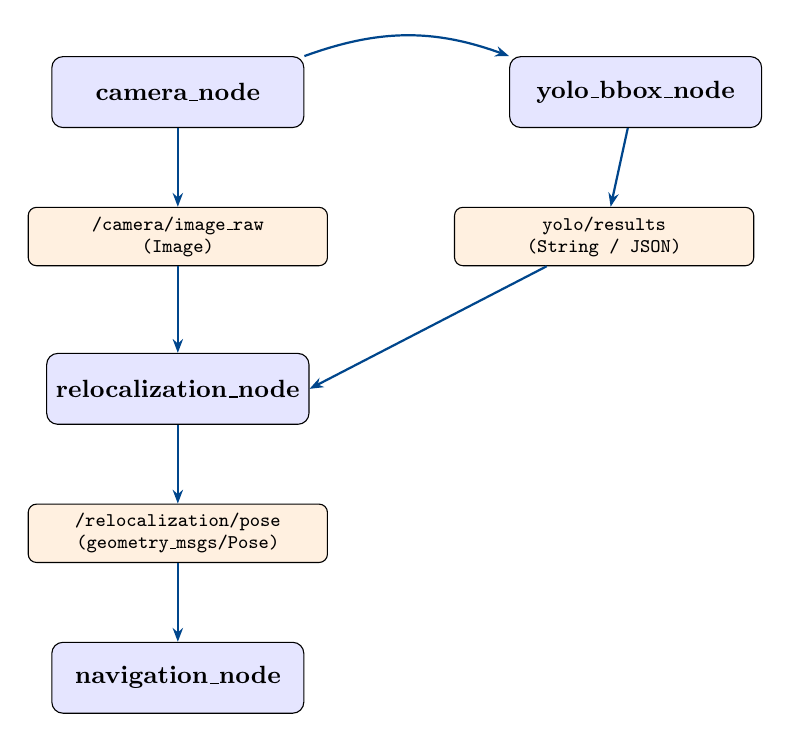
\begin{tikzpicture}[
  node distance=1.2cm and 2.2cm,
  box/.style={draw, rounded corners=4pt, fill=blue!10, minimum width=3.2cm,
              minimum height=0.9cm, align=center, font=\small\bfseries},
  topic/.style={draw, rounded corners=3pt, fill=orange!12, minimum width=3.8cm,
                minimum height=0.7cm, align=center, font=\scriptsize\ttfamily},
  arr/.style={-{Stealth[length=5pt]}, thick, color=hdrblue}
]
  \node[box] (cam)    {camera\_node};
  \node[box, right=2.6cm of cam] (yolo)  {yolo\_bbox\_node};

  \node[topic, below=1.0cm of cam]  (imgtopic) {/camera/image\_raw\\(Image)};
  \node[topic, right=1.6cm of imgtopic] (ytopic) {yolo/results\\(String / JSON)};

  \node[box, below=1.1cm of imgtopic]  (reloc) {relocalization\_node};

  \node[topic, below=1.0cm of reloc] (ptopic) {/relocalization/pose\\(geometry\_msgs/Pose)};

  \node[box, below=1.0cm of ptopic]  (nav)   {navigation\_node};

  \draw[arr] (cam) -- (imgtopic);
  \draw[arr] (imgtopic) -- (reloc);
  \draw[arr] (cam.north east) to[bend left=20] (yolo.north west);
  \draw[arr] (yolo) -- (ytopic);
  \draw[arr] (ytopic) -- (reloc.east);
  \draw[arr] (reloc) -- (ptopic);
  \draw[arr] (ptopic) -- (nav);
\end{tikzpicture}
\caption{ROS\,2 node graph. The \texttt{relocalization\_node} fuses raw image data
         with YOLO semantic detections to produce a weighted pose estimate.}
\label{fig:nodegraph}
\end{figure}

%% ═══════════════════════════════════════════════════════════════════════════════
\section{Camera Model}
%% ═══════════════════════════════════════════════════════════════════════════════

The system uses a standard \textbf{pinhole camera model}. A 3-D world point
$\mathbf{X}^w$ is first transformed into camera coordinates
$\mathbf{P}_c = [X_c,\,Y_c,\,Z_c]^\top$ by the current pose $\mathbf{T}_{cw}$,
then projected onto the image plane:

\begin{formulabox}{Perspective Projection}
\begin{equation}
  u = f_x\,\frac{X_c}{Z_c} + c_x, \qquad v = f_y\,\frac{Y_c}{Z_c} + c_y
  \label{eq:proj}
\end{equation}
\end{formulabox}

\begin{figure}[H]
\centering
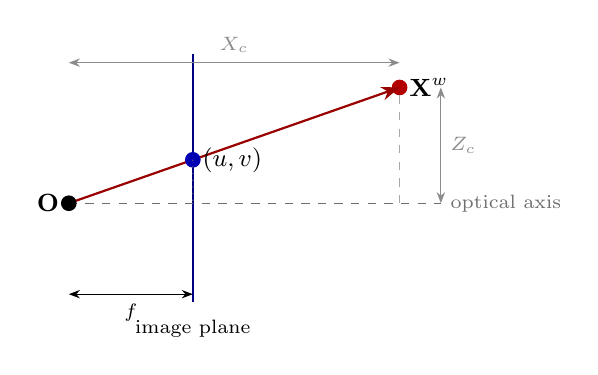
\begin{tikzpicture}[scale=1.05]
  % Image plane
  \fill[blue!5] (1.5,-1.2) rectangle (1.52,1.8);
  \draw[thick,blue!50!black] (1.5,-1.2) -- (1.5,1.8);
  \node[font=\scriptsize, below] at (1.5,-1.3) {image plane};

  % Optical axis
  \draw[dashed,cgray] (0,0) -- (4.5,0) node[right,font=\scriptsize,cgray]{optical axis};

  % World point
  \coordinate (Xw) at (4.0,1.4);
  \filldraw[red!70!black] (Xw) circle (2.5pt);
  \node[right, font=\small] at (Xw) {$\mathbf{X}^w$};

  % Ray
  \draw[-{Stealth},thick,red!60!black] (0,0) -- (Xw);

  % Projected point
  \coordinate (proj) at (1.5, 0.525);
  \filldraw[blue!70!black] (proj) circle (2.5pt);
  \node[right, font=\small] at (proj) {$(u,v)$};
  \draw[dotted,cgray] (proj) -- (1.5,0);

  % Camera centre
  \filldraw[black] (0,0) circle (2.5pt) node[left,font=\small]{$\mathbf{O}$};

  % Focal length arrow
  \draw[{Stealth[length=4pt]}-{Stealth[length=4pt]}] (0,-1.1) -- node[below,font=\scriptsize]{$f$} (1.5,-1.1);

  % Zc / Xc labels
  \draw[dashed,cgray!60] (4.0,0) -- (4.0,1.4);
  \draw[{Stealth[length=4pt]}-{Stealth[length=4pt]},cgray!80] (0,1.7) -- node[above,font=\scriptsize]{$X_c$} (4.0,1.7);
  \draw[{Stealth[length=4pt]}-{Stealth[length=4pt]},cgray!80] (4.5,0) -- node[right,font=\scriptsize]{$Z_c$} (4.5,1.4);
\end{tikzpicture}
\caption{Pinhole projection geometry. The world point $\mathbf{X}^w$ projects to pixel
         $(u,v)$ at the intersection of the ray from optical centre $\mathbf{O}$ and
         the image plane.}
\label{fig:pinhole}
\end{figure}

\begin{table}[H]
\centering
\caption{Camera intrinsics used --- TUM FR3 dataset (\texttt{tum\_fr3.yaml})}
\begin{tabular}{llrl}
\toprule
YAML key & Symbol & Value & Description \\
\midrule
\texttt{Camera1.fx} & $f_x$ & 535.4 & Horizontal focal length (px) \\
\texttt{Camera1.fy} & $f_y$ & 539.2 & Vertical focal length (px) \\
\texttt{Camera1.cx} & $c_x$ & 320.1 & Horizontal principal point (px) \\
\texttt{Camera1.cy} & $c_y$ & 247.6 & Vertical principal point (px) \\
\texttt{Camera.width}  & $W$ & 640 & Image width (px) \\
\texttt{Camera.height} & $H$ & 480 & Image height (px) \\
\texttt{Camera1.k1--k3} & --- & 0.0 & Radial distortion (none) \\
\bottomrule
\end{tabular}
\end{table}

%% ═══════════════════════════════════════════════════════════════════════════════
\section{ORB Feature Extraction and Candidate Matching}
%% ═══════════════════════════════════════════════════════════════════════════════

Each frame is processed in three steps before any pose computation:

\begin{enumerate}
  \item \textbf{ORB extraction.} 1000 oriented FAST corners are detected across an
        8-level image pyramid (scale factor 1.2) and described with 256-bit binary
        ORB descriptors.

  \item \textbf{Bag-of-Words retrieval.} The frame's BoW vector is compared against
        all map keyframes. Keyframes whose cosine similarity exceeds
        \texttt{BowSimilarityThreshold}\,=\,0.018 become \emph{candidates}.

  \item \textbf{Descriptor matching.} ORB descriptors of the query frame are matched
        to each candidate keyframe, yielding a set of 2D--3D correspondences
        $\{(\mathbf{p}_i,\,\mathbf{X}^w_i)\}_{i=1}^{n}$.
\end{enumerate}

\begin{table}[H]
\centering
\caption{ORB extractor and relocalization parameters (\texttt{tum\_fr3.yaml})}
\begin{tabular}{lrl}
\toprule
Parameter & Value & Description \\
\midrule
\texttt{ORBextractor.nFeatures}            & 1000  & Keypoints extracted per frame \\
\texttt{ORBextractor.scaleFactor}          & 1.2   & Pyramid level scale ratio \\
\texttt{ORBextractor.nLevels}              & 8     & Number of pyramid levels \\
\texttt{ORBextractor.iniThFAST}            & 20    & Initial FAST response threshold \\
\texttt{ORBextractor.minThFAST}            & 7     & Fallback FAST threshold \\
\texttt{Relocalization.BowSimilarityThreshold} & 0.018 & Minimum BoW cosine similarity \\
\texttt{Relocalization.MinInliers}         & 15    & Minimum inliers for pose acceptance \\
\bottomrule
\end{tabular}
\end{table}

%% ═══════════════════════════════════════════════════════════════════════════════
\section{YOLO Detection Integration}
%% ═══════════════════════════════════════════════════════════════════════════════

\subsection{Detection Message Format}

The \texttt{yolo\_bbox\_node} runs YOLOv8 inference on each incoming frame (resized to
$640\times480$) and publishes results as a JSON string on \texttt{yolo/results}:

\begin{lstlisting}[style=json,
  caption={JSON payload on \texttt{yolo/results} (\texttt{yolo\_bbox\_video.py})}]
{
  "frame_id": 42,
  "detections": [
    {
      "cls_id": 164,
      "conf_score": 0.92,
      "bbox_coords": { "x1": 100, "y1": 200, "x2": 350, "y2": 450 }
    }
  ]
}
\end{lstlisting}

\begin{notebox}
Class ID \textbf{164 = door} in the YOLOv8 Open Images V7 vocabulary. Doors are
chosen because they are \emph{permanent}, \emph{geometrically stable}, and
\emph{visually distinctive} --- ideal anchor points for relocalization.
\end{notebox}

\subsection{ROS\,2 Subscription and Parsing}

The relocalization node subscribes to \texttt{yolo/results} with a mutex-protected
callback. Parsed bounding boxes are stored in \texttt{latest\_bboxes\_}:

\begin{lstlisting}[style=cpp,
  caption={\texttt{yoloCallback()} ---
           \texttt{relocalization\_node.cpp}, lines\,450--467}]
void yoloCallback(const std_msgs::msg::String::SharedPtr msg)
{
    try {
        auto data = nlohmann::json::parse(msg->data);
        std::lock_guard<std::mutex> lock(bbox_mutex_);
        latest_bboxes_.clear();

        for (const auto &det : data["detections"])
        {
            int x1 = det["bbox_coords"]["x1"].get<int>();
            int y1 = det["bbox_coords"]["y1"].get<int>();
            int x2 = det["bbox_coords"]["x2"].get<int>();
            int y2 = det["bbox_coords"]["y2"].get<int>();

            latest_bboxes_.push_back({
                det["cls_id"].get<int>(),
                cv::Rect(x1, y1, x2 - x1, y2 - y1)
            });
        }
    }
    catch (const nlohmann::json::exception &e) {
        RCLCPP_WARN(get_logger(), "YOLO parse error: %s", e.what());
    }
}
\end{lstlisting}

\begin{notebox}
\texttt{bbox\_mutex\_} ensures thread safety between the YOLO ROS\,2 callback (which
writes \texttt{latest\_bboxes\_}) and the main processing loop (which reads it).
\end{notebox}

\subsection{Bounding Box Coordinate Scaling}

YOLO always outputs coordinates at $640\times480$. Before use, these are scaled to the
processing resolution ($W_\text{proc}\times H_\text{proc}$, also $640\times480$ in the
TUM FR3 configuration, but handled generically):

\begin{formulabox}{Bbox Scaling Factors}
\begin{equation}
  s_x = \frac{W_{\text{proc}}}{640}, \qquad s_y = \frac{H_{\text{proc}}}{480}
  \label{eq:scale}
\end{equation}
Each bbox corner $(x,y)$ maps to $(s_x x,\; s_y y)$.
\end{formulabox}

\begin{figure}[H]
\centering
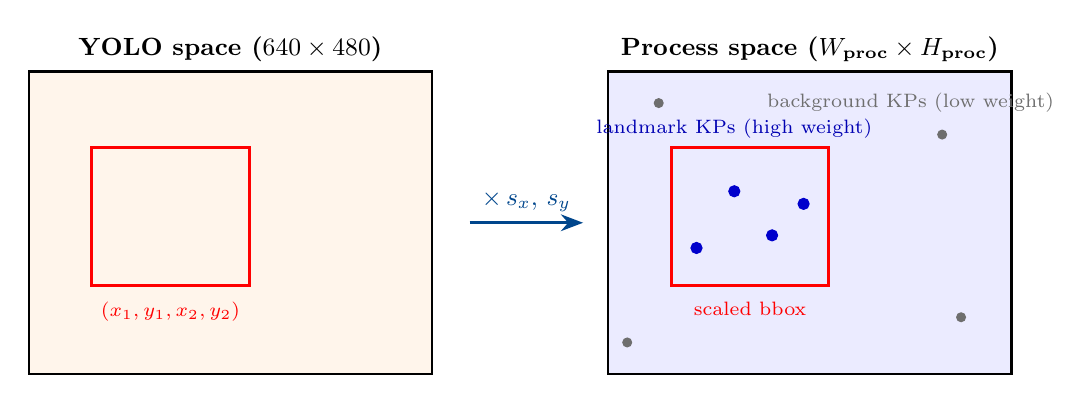
\begin{tikzpicture}[scale=0.80]
  % --- YOLO space ---
  \fill[orange!8] (0,0) rectangle (6.4,4.8);
  \draw[thick] (0,0) rectangle (6.4,4.8);
  \node[above, font=\small\bfseries] at (3.2,4.8) {YOLO space ($640\times480$)};

  % YOLO bbox
  \draw[red, very thick] (1.0,1.4) rectangle (3.5,3.6);
  \node[red, font=\scriptsize, below] at (2.25,1.3) {$(x_1,y_1,x_2,y_2)$};

  % Arrow
  \draw[-{Stealth[length=8pt]}, very thick, hdrblue]
    (7.0,2.4) -- node[above,font=\small]{$\times\,s_x,\,s_y$} (8.8,2.4);

  % --- Process space ---
  \fill[blue!8] (9.2,0) rectangle (15.6,4.8);
  \draw[thick] (9.2,0) rectangle (15.6,4.8);
  \node[above, font=\small\bfseries] at (12.4,4.8)
    {Process space ($W_\text{proc}\times H_\text{proc}$)};

  % Scaled bbox
  \draw[red, very thick] (10.2,1.4) rectangle (12.7,3.6);
  \node[red, font=\scriptsize, below] at (11.45,1.3) {scaled bbox};

  % ORB keypoints inside
  \foreach \x/\y in {10.6/2.0, 11.2/2.9, 11.8/2.2, 12.3/2.7} {
    \filldraw[blue!80!black] (\x,\y) circle (2.5pt);
  }
  \node[blue!70!black, font=\scriptsize] at (11.2,3.9) {landmark KPs (high weight)};

  % Background keypoints
  \foreach \x/\y in {9.5/0.5, 14.8/0.9, 14.5/3.8, 10.0/4.3} {
    \filldraw[cgray] (\x,\y) circle (2pt);
  }
  \node[cgray, font=\scriptsize] at (14.0,4.3) {background KPs (low weight)};
\end{tikzpicture}
\caption{YOLO bboxes are scaled from $640\times480$ to the processing resolution.
         ORB keypoints inside the scaled box become \emph{landmark keypoints} with
         high weight; all others are \emph{background}.}
\label{fig:bboxscale}
\end{figure}

%% ═══════════════════════════════════════════════════════════════════════════════
\section{Landmark Segmentation}
%% ═══════════════════════════════════════════════════════════════════════════════

After scaling, the node iterates over all ORB matches and assigns each matched 2-D
point to a \texttt{LandmarkRegion} when it falls inside a scaled bounding box. A
pixel proximity tolerance of $0.5$\,px is used for floating-point safety:

\begin{lstlisting}[style=cpp,
  caption={Landmark segmentation ---
           \texttt{relocalization\_node.cpp}, lines\,171--203}]
const float sx = (float)processSize.width  / 640.0f;
const float sy = (float)processSize.height / 480.0f;

for (const auto &det : bboxes)
{
    Relocalization::LandmarkRegion region;
    region.cls_id = det.cls_id;
    region.bbox   = cv::Rect(
        (int)(det.bbox.x      * sx), (int)(det.bbox.y      * sy),
        (int)(det.bbox.width  * sx), (int)(det.bbox.height * sy));

    for (const auto &kp : result.queryKeypoints)
    {
        if (region.bbox.contains(cv::Point((int)kp.pt.x, (int)kp.pt.y)))
            region.keypoints.push_back(kp);
    }

    result.landmarkRegions.push_back(std::move(region));
}
\end{lstlisting}

The \texttt{LandmarkRegion} struct groups all keypoints belonging to one detection:

\begin{lstlisting}[style=cpp,
  caption={\texttt{LandmarkRegion} struct ---
           \texttt{relocalization.h}, lines\,21--27}]
struct LandmarkRegion
{
    int                        cls_id;     // YOLO class ID (e.g. 164 = door)
    cv::Rect                   bbox;       // Bounding box (process resolution)
    std::vector<cv::KeyPoint>  keypoints;  // ORB keypoints inside the bbox
};
\end{lstlisting}

%% ═══════════════════════════════════════════════════════════════════════════════
\section{Semantic Weight Assignment}
%% ═══════════════════════════════════════════════════════════════════════════════

\subsection{Weight Hierarchy}

Three tiers of trust are defined based on YOLO class:

\begin{figure}[H]
\centering
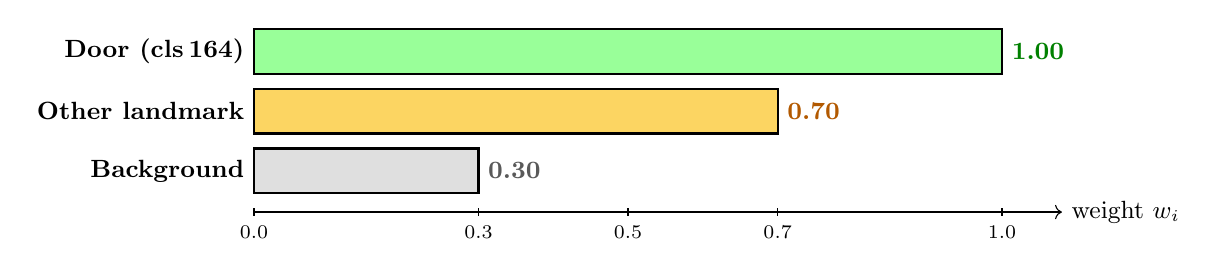
\begin{tikzpicture}[scale=0.95]
  % Background tier
  \fill[gray!25]              (0.0,0.00) rectangle (0.3*10,0.60);
  % Other landmark tier
  \fill[yellow!50!orange!60]  (0.0,0.80) rectangle (0.7*10,1.40);
  % Door tier
  \fill[green!40]             (0.0,1.60) rectangle (1.0*10,2.20);

  \draw[thick] (0,0.00) rectangle (0.3*10,0.60);
  \draw[thick] (0,0.80) rectangle (0.7*10,1.40);
  \draw[thick] (0,1.60) rectangle (1.0*10,2.20);

  % Axis
  \draw[->] (0,-0.25) -- (10.8,-0.25) node[right,font=\small]{weight $w_i$};
  \foreach \x/\l in {0/0.0, 3/0.3, 5/0.5, 7/0.7, 10/1.0}
    \draw (\x,-0.20) -- (\x,-0.30) node[below,font=\scriptsize]{\l};

  % Labels (left)
  \node[left, font=\small\bfseries] at (0, 0.30) {Background};
  \node[left, font=\small\bfseries] at (0, 1.10) {Other landmark};
  \node[left, font=\small\bfseries] at (0, 1.90) {Door (cls\,164)};

  % Value labels (right of bar)
  \node[right, font=\small\bfseries, gray!70!black]       at (3.0,0.30)  {0.30};
  \node[right, font=\small\bfseries, orange!70!black]     at (7.0,1.10)  {0.70};
  \node[right, font=\small\bfseries, green!50!black]      at (10.0,1.90) {1.00};
\end{tikzpicture}
\caption{Semantic weight tiers. Door keypoints receive maximum weight (1.00);
         other detected landmarks get 0.70; background keypoints get 0.30.}
\label{fig:weightbars}
\end{figure}

\subsection{Semantic Weight Function}

\begin{lstlisting}[style=cpp,
  caption={\texttt{getSemanticWeight()} ---
           \texttt{relocalization.cpp}, lines\,1113--1121}]
static float getSemanticWeight(int cls_id)
{
    switch (cls_id)
    {
        case 164: return 1.0f;  // Door -- highly permanent landmark
        default:  return 0.7f;  // Any other detected object class
    }
}
\end{lstlisting}

\subsection{Weight Assignment to All Matches}

\begin{lstlisting}[style=cpp,
  caption={\texttt{assignWeightsFromLandmarks()} ---
           \texttt{relocalization.cpp}, lines\,1170--1194}]
std::vector<float> RelocalizationModule::assignWeightsFromLandmarks(
    const std::vector<cv::Point2f>   &matched2DPoints,
    const std::vector<LandmarkRegion>&landmarkRegions,
    float permanentWeight,   // = 1.0f at call site
    float backgroundWeight)  // = 0.3f at call site
{
    // Initialise every point to background level
    std::vector<float> weights(matched2DPoints.size(), backgroundWeight);

    for (size_t i = 0; i < matched2DPoints.size(); ++i)
    {
        for (const auto &region : landmarkRegions)
        {
            for (const auto &kp : region.keypoints)
            {
                // Pixel proximity: 0.5 px tolerance
                if (std::abs(kp.pt.x - matched2DPoints[i].x) < 0.5f &&
                    std::abs(kp.pt.y - matched2DPoints[i].y) < 0.5f)
                {
                    float w = getSemanticWeight(region.cls_id) * permanentWeight;
                    weights[i] = std::max(weights[i], w);  // keep the highest
                    break;
                }
            }
        }
    }
    return weights;
}
\end{lstlisting}

\begin{table}[H]
\centering
\caption{Weight assignment parameters
         (\texttt{relocalization\_node.cpp}, lines\,209--215)}
\begin{tabular}{llrl}
\toprule
Variable & Type & Value & Role \\
\midrule
\texttt{permanentWeight}  & \texttt{float} & 1.0 & Multiplier on \texttt{getSemanticWeight()} result \\
\texttt{backgroundWeight} & \texttt{float} & 0.3 & Default weight outside any bbox \\
Proximity tolerance       & \texttt{float} & 0.5\,px & Max distance to match a 2D point to a keypoint \\
\bottomrule
\end{tabular}
\end{table}

%% ═══════════════════════════════════════════════════════════════════════════════
\section{Weighted PnP --- Mathematical Formulation}
%% ═══════════════════════════════════════════════════════════════════════════════

\subsection{Objective Function}

Given $n$ 2D--3D correspondences $\{(\mathbf{p}_i,\,\mathbf{X}^w_i)\}$ and
per-point weights $\{w_i\}$, the goal is to find the camera pose
$\mathbf{T}_{cw} \in SE(3)$ that minimises the \emph{weighted reprojection error}:

\begin{formulabox}{Weighted Cost Function}
\begin{equation}
  E(\xi) = \sum_{i=1}^{n} w_i\,\|\mathbf{r}_i\|^2
         = \sum_{i=1}^{n} w_i\,\bigl\|\mathbf{p}_i - \pi\!\left(
             \mathbf{T}_{cw} \cdot \mathbf{X}^w_i\right)\bigr\|^2
  \label{eq:cost}
\end{equation}
\vspace{2pt}
\begin{tabular}{ll}
  $\xi \in \mathfrak{se}(3)$ & 6-D Lie algebra element (3 translation $+$ 3 rotation) \\
  $w_i \in \{0.30,\,0.70,\,1.00\}$ & Semantic weight \\
  $\mathbf{p}_i \in \mathbb{R}^2$ & Observed 2-D keypoint \\
  $\pi(\cdot)$ & Perspective projection (Eq.~\ref{eq:proj}) \\
  $\mathbf{T}_{cw} \in SE(3)$ & Camera-to-world transformation \\
  $\mathbf{X}^w_i \in \mathbb{R}^3$ & Map 3-D point \\
  $\mathbf{r}_i \in \mathbb{R}^2$ & Reprojection residual \\
\end{tabular}
\end{formulabox}

\subsection{SE(3) Lie Group Representation}

The pose is stored as a Sophus \texttt{SE3d} object. Rather than operating in
Euclidean space, updates are applied on the manifold via the \emph{exponential map}
(left perturbation):

\begin{formulabox}{Pose Update via Exponential Map}
\begin{equation}
  \mathbf{T}_{\text{new}} = \exp(\delta\xi)\cdot\mathbf{T}_{cw}, \qquad
  \delta\xi \in \mathbb{R}^6
  \label{eq:expmap}
\end{equation}
$\delta\xi = [\delta\mathbf{t}^\top,\;\delta\boldsymbol{\omega}^\top]^\top$:
3 translational + 3 rotational increments.
\end{formulabox}

\subsection{Weight Normalisation}

Before optimization, all weights are normalised so their mean equals 1. This keeps
the scale of the Hessian $\mathbf{H}$ consistent across frames with different
numbers of correspondences:

\begin{formulabox}{Weight Normalisation}
\begin{equation}
  \bar{w} = \frac{1}{n}\sum_{i=1}^{n} w_i, \qquad
  \hat{w}_i = \frac{w_i}{\bar{w}}
  \label{eq:wnorm}
\end{equation}
\end{formulabox}

\begin{lstlisting}[style=cpp,
  caption={Weight normalisation ---
           \texttt{relocalization.cpp}, lines\,1218--1226}]
float w_sum = 0.0f;
for (float w : weights) w_sum += w;
float w_mean = w_sum / n;

std::vector<double> w_norm(n);
for (int i = 0; i < n; ++i)
    w_norm[i] = (double)(weights[i] / w_mean);
\end{lstlisting}

%% ═══════════════════════════════════════════════════════════════════════════════
\section{Projection Jacobian}
%% ═══════════════════════════════════════════════════════════════════════════════

The Gauss--Newton solver needs the Jacobian of the 2-D residual
$\mathbf{r}_i$ with respect to the 6-D perturbation $\delta\xi$:

\begin{equation}
  \mathbf{J}_i
    = \frac{\partial\mathbf{r}_i}{\partial\delta\xi}
    = \frac{\partial[u,v]^\top}{\partial[\delta\mathbf{t}^\top,\,\delta\boldsymbol{\omega}^\top]}
    \in \mathbb{R}^{2\times6}
\end{equation}

Let $\mathbf{P}_c = [X_c,\,Y_c,\,Z_c]^\top$ be the point in camera coordinates,
$\zeta_1 = Z_c^{-1}$, $\zeta_2 = Z_c^{-2}$.
The full Jacobian under the left SE(3) perturbation model is:

\begin{formulabox}{$2\times6$ Projection Jacobian}
\begin{equation}
\mathbf{J} = \begin{pmatrix}
  f_x\zeta_1 & 0 & -f_x X_c\zeta_2 &
    -f_x X_c Y_c\zeta_2 & f_x(1+X_c^2\zeta_2) & -f_x Y_c\zeta_1 \\[4pt]
  0 & f_y\zeta_1 & -f_y Y_c\zeta_2 &
    -f_y(1+Y_c^2\zeta_2) & f_y X_c Y_c\zeta_2 &  f_y X_c\zeta_1
\end{pmatrix}
\label{eq:jac}
\end{equation}
Columns: $[\partial/\partial t_x,\;\partial/\partial t_y,\;\partial/\partial t_z,\;
\partial/\partial\omega_x,\;\partial/\partial\omega_y,\;\partial/\partial\omega_z]$.
\end{formulabox}

\begin{lstlisting}[style=cpp,
  caption={\texttt{computeProjectionJacobian()} ---
           \texttt{relocalization.cpp}, lines\,1124--1147}]
Eigen::Matrix<double, 2, 6> RelocalizationModule::computeProjectionJacobian(
    const Eigen::Vector3d &Pc, double fx, double fy)
{
    double Xc = Pc(0), Yc = Pc(1), Zc = Pc(2);
    double Zc_inv  = 1.0 / Zc;
    double Zc_inv2 = Zc_inv * Zc_inv;

    Eigen::Matrix<double, 2, 6> J;

    // Row 0: du/d(delta_xi) = [du/dt | du/domega]
    J(0, 0) =  fx * Zc_inv;
    J(0, 1) =  0.0;
    J(0, 2) = -fx * Xc * Zc_inv2;
    J(0, 3) = -fx * Xc * Yc * Zc_inv2;
    J(0, 4) =  fx + fx * Xc * Xc * Zc_inv2;
    J(0, 5) = -fx * Yc * Zc_inv;

    // Row 1: dv/d(delta_xi) = [dv/dt | dv/domega]
    J(1, 0) =  0.0;
    J(1, 1) =  fy * Zc_inv;
    J(1, 2) = -fy * Yc * Zc_inv2;
    J(1, 3) = -(fy + fy * Yc * Yc * Zc_inv2);
    J(1, 4) =  fy * Xc * Yc * Zc_inv2;
    J(1, 5) =  fy * Xc * Zc_inv;

    return J;
}
\end{lstlisting}

%% ═══════════════════════════════════════════════════════════════════════════════
\section{Levenberg--Marquardt Solver}
%% ═══════════════════════════════════════════════════════════════════════════════

\subsection{Weighted Normal Equations}

At each iteration the weighted Gauss--Newton system is assembled and damped:

\begin{formulabox}{Weighted Normal Equations}
\begin{align}
  \mathbf{H}         &= \sum_{i=1}^{n} \hat{w}_i\,\mathbf{J}_i^\top\mathbf{J}_i
                        \;\in\mathbb{R}^{6\times6}
                        \label{eq:H} \\[4pt]
  \mathbf{b}         &= \sum_{i=1}^{n} \hat{w}_i\,\mathbf{J}_i^\top\mathbf{r}_i
                        \;\in\mathbb{R}^{6}
                        \label{eq:b} \\[4pt]
  \mathbf{H}_\lambda &= \mathbf{H} + \lambda\,\mathrm{diag}(\mathbf{H}),
  \qquad
  \mathbf{H}_\lambda\,\delta\xi = \mathbf{b}
  \label{eq:lm}
\end{align}
The damped system (Eq.~\ref{eq:lm}) is solved with LDLT decomposition.
\end{formulabox}

The LM damping parameter $\lambda$ adapts every iteration:
\[
  \text{if } E_{\text{new}} < E_{\text{old}} \;\Rightarrow\; \lambda \mathrel{/}= 10
  \quad(\text{more Newton-like})
\]
\[
  \text{if } E_{\text{new}} \geq E_{\text{old}} \;\Rightarrow\; \lambda \mathrel{*}= 10
  \quad(\text{more gradient-descent-like})
\]

\subsection{Core Optimization Loop}

\begin{lstlisting}[style=cpp,
  caption={LM core loop ---
           \texttt{relocalization.cpp}, lines\,1254--1302 (abridged)}]
Sophus::SE3d T_cw(R_e, t_e);  // warm-started from EPnP
double lambda = 1e-3;
double cost   = std::numeric_limits<double>::max();

for (int iter = 0; iter < maxIterations; ++iter)
{
    Eigen::Matrix<double,6,6> H = Eigen::Matrix<double,6,6>::Zero();
    Eigen::Matrix<double,6,1> b = Eigen::Matrix<double,6,1>::Zero();
    double new_cost = 0.0;

    for (int i = 0; i < n; ++i)
    {
        Eigen::Vector3d Xw(points3D[i].x, points3D[i].y, points3D[i].z);
        Eigen::Vector3d Pc = T_cw * Xw;
        if (Pc(2) <= 0) continue;  // skip points behind camera

        double u_proj = fx * Pc(0) / Pc(2) + cx;
        double v_proj = fy * Pc(1) / Pc(2) + cy;
        Eigen::Vector2d r(points2D[i].x - u_proj, points2D[i].y - v_proj);

        Eigen::Matrix<double,2,6> J = computeProjectionJacobian(Pc, fx, fy);
        double w  = w_norm[i];       // normalised semantic weight
        H        += w * J.transpose() * J;
        b        += w * J.transpose() * r;
        new_cost += w * r.squaredNorm();
    }

    // Levenberg-Marquardt damping
    Eigen::Matrix<double,6,6> H_d = H;
    for (int k = 0; k < 6; ++k)
        H_d(k,k) += lambda * H(k,k);

    Eigen::Matrix<double,6,1> delta = H_d.ldlt().solve(b);
    Sophus::SE3d T_new = Sophus::SE3d::exp(delta) * T_cw;

    if (new_cost < cost) { T_cw = T_new; cost = new_cost; lambda /= 10.0; }
    else                 {                                 lambda *= 10.0; }

    if (delta.norm() < convergenceThreshold) break;
}
\end{lstlisting}

\subsection{Solver Parameters}

\begin{table}[H]
\centering
\caption{\texttt{solvePnPWeighted()} parameters
         (\texttt{relocalization.h}, lines\,87--93)}
\begin{tabular}{llrl}
\toprule
Parameter & Type & Default & Meaning \\
\midrule
\texttt{maxIterations}        & \texttt{int}    & 100   & Maximum LM iterations \\
\texttt{convergenceThreshold} & \texttt{double} & 1e-6  & Stop when $\|\delta\xi\| <$ this \\
\texttt{inlierThresholdPx}    & \texttt{float}  & 2.0   & Reprojection cutoff for inlier count (px) \\
$\lambda_0$                   & \texttt{double} & 1e-3  & Initial LM damping \\
\bottomrule
\end{tabular}
\end{table}

\begin{definitionbox}{EPnP Warm-Start}
Before the LM loop, \texttt{solvePnPWeighted()} calls \texttt{cv::solvePnP} with flag
\texttt{SOLVEPNP\_EPNP} to obtain an initial $\mathbf{T}_{cw}$. This prevents
cold-start divergence and typically halves the number of LM iterations needed.
\end{definitionbox}

%% ═══════════════════════════════════════════════════════════════════════════════
\section{Result Structure and Metrics}
%% ═══════════════════════════════════════════════════════════════════════════════

The solver returns a \texttt{WeightedPnPResult} struct:

\begin{lstlisting}[style=cpp,
  caption={\texttt{WeightedPnPResult} ---
           \texttt{relocalization.h}, lines\,29--41}]
struct WeightedPnPResult
{
    bool        success;                   // converged with >= MinInliers inliers
    cv::Point3f position;                  // camera position in world frame
    int         numInliers;               // points with reproj. error < 2.0 px
    int         totalCorrespondences;     // total matched 2D-3D pairs
    float       meanReprojectionError;    // unweighted mean reproj. error (px)
    float       weightedReprojectionError;// weighted cost / n
    int         iterations;              // LM iterations to convergence
    std::vector<int> inlierIndices;       // accepted inlier indices
    cv::Mat     rvec;                     // Rodrigues rotation vector
    cv::Mat     tvec;                     // translation vector
};
\end{lstlisting}

The node also writes a per-frame CSV (\texttt{comparison\_log.csv}) to enable
offline comparison of weighted vs.\ standard RANSAC-PnP:

\begin{table}[H]
\centering
\caption{CSV log columns for weighted vs.\ standard PnP comparison}
\begin{tabular}{ll}
\toprule
Column & Meaning \\
\midrule
\texttt{std\_inliers}         & Standard RANSAC-PnP inlier count \\
\texttt{wpnp\_inliers}        & Weighted-PnP inlier count \\
\texttt{wpnp\_reproj\_px}     & Weighted-PnP mean reprojection error (px) \\
\texttt{wpnp\_weighted\_cost} & Final cost $E(\xi)$ (Eq.~\ref{eq:cost}) \\
\texttt{pose\_delta\_m}       & Translation difference vs.\ standard PnP (m) \\
\texttt{wpnp\_iterations}     & LM iterations used \\
\bottomrule
\end{tabular}
\end{table}

%% ═══════════════════════════════════════════════════════════════════════════════
\section{Full Algorithm Flowchart}
%% ═══════════════════════════════════════════════════════════════════════════════

\begin{figure}[H]
\centering
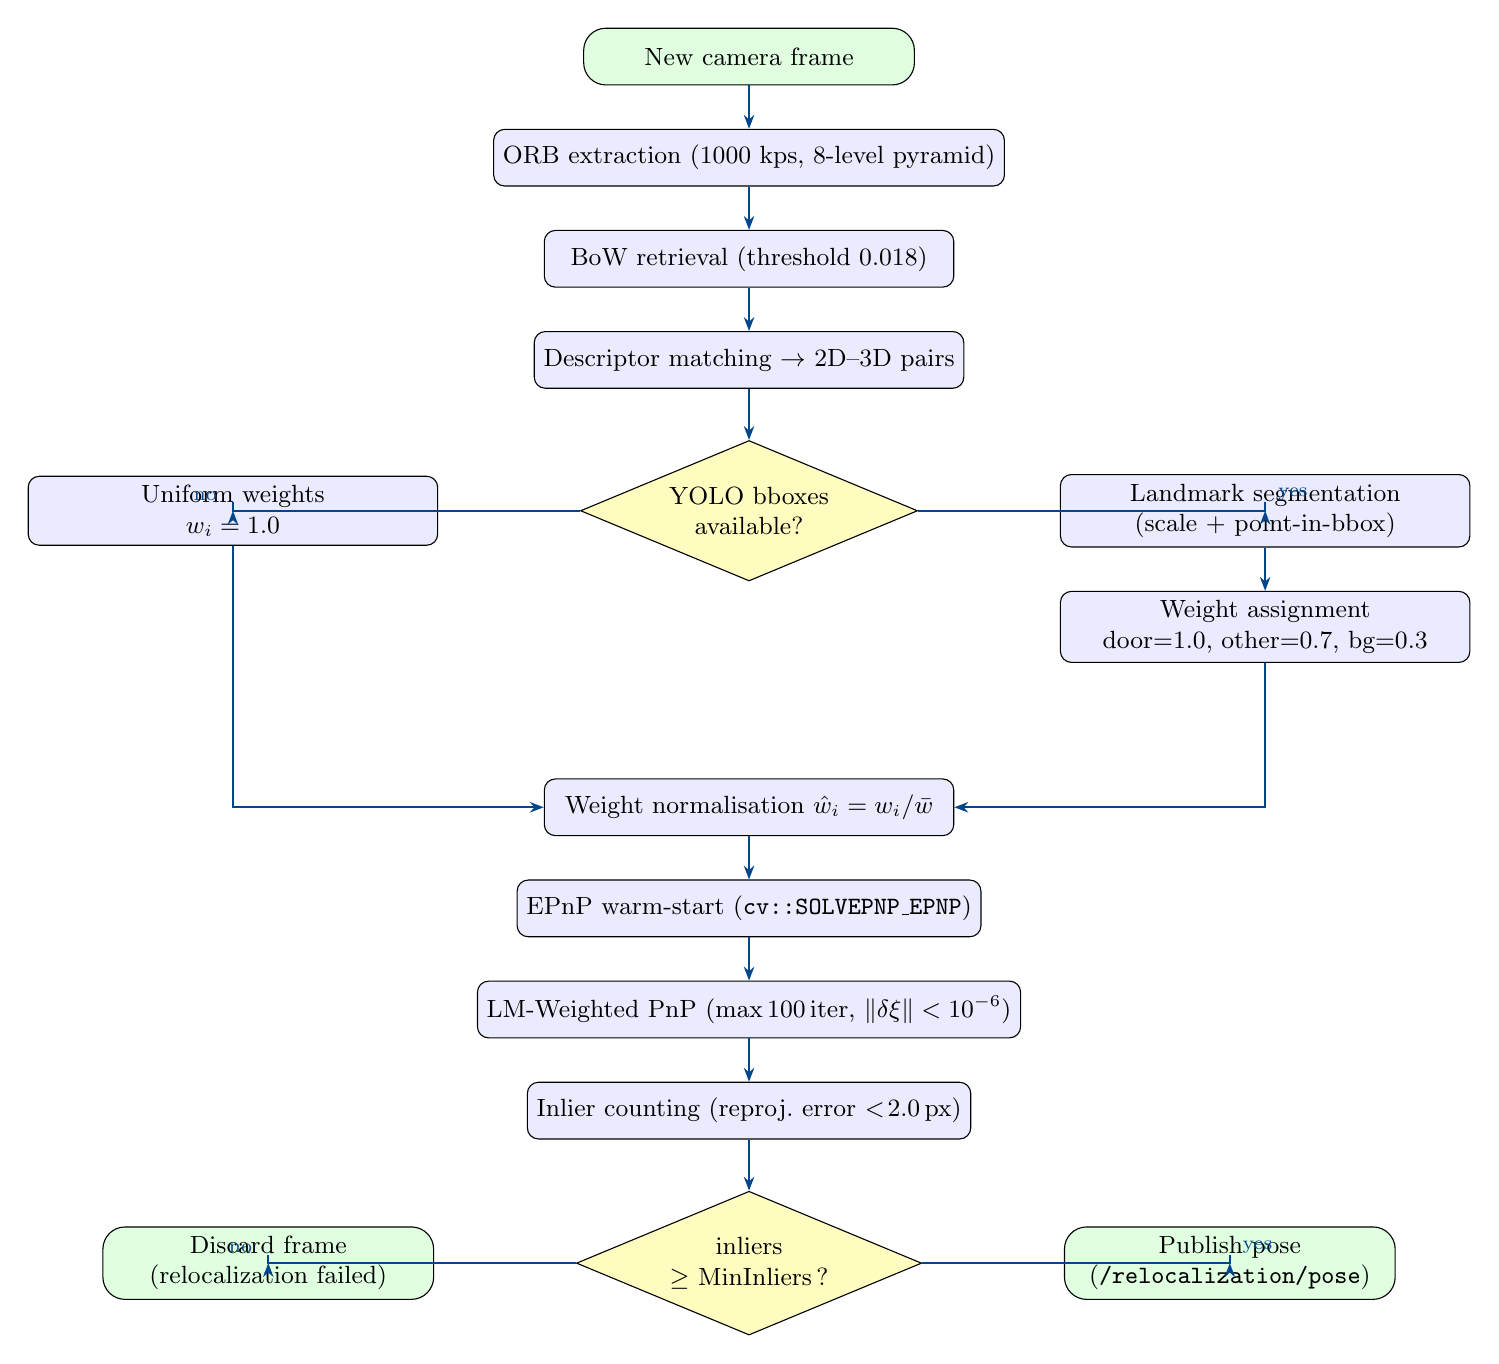
\begin{tikzpicture}[
  node distance=0.55cm and 0.4cm,
  block/.style={draw, rounded corners=4pt, fill=blue!8, minimum width=5.2cm,
                minimum height=0.72cm, align=center, font=\small},
  decision/.style={draw, diamond, aspect=2.4, fill=yellow!25,
                   minimum width=4.0cm, minimum height=0.82cm,
                   align=center, font=\small},
  io/.style={draw, rounded corners=8pt, fill=green!12,
             minimum width=4.2cm, minimum height=0.72cm,
             align=center, font=\small},
  arr/.style={-{Stealth[length=5pt]}, thick, hdrblue}
]

\node[io]      (frame)  {New camera frame};
\node[block, below=of frame]   (orb)   {ORB extraction (1000 kps, 8-level pyramid)};
\node[block, below=of orb]     (bow)   {BoW retrieval (threshold 0.018)};
\node[block, below=of bow]     (match) {Descriptor matching $\to$ 2D--3D pairs};
\node[decision, below=0.65cm of match] (hasbbox) {YOLO bboxes\\available?};

% YES branch (right)
\node[block, right=1.8cm of hasbbox, yshift=0.0cm]  (seg)    {Landmark segmentation\\(scale + point-in-bbox)};
\node[block, below=of seg]                            (wassign){Weight assignment\\door=1.0, other=0.7, bg=0.3};

% NO branch (left)
\node[block, left=1.8cm of hasbbox]   (unif)   {Uniform weights\\$w_i = 1.0$};

% Merge
\node[block, below=2.5cm of hasbbox]  (norm)   {Weight normalisation $\hat{w}_i = w_i/\bar{w}$};
\node[block, below=of norm]            (epnp)   {EPnP warm-start (\texttt{cv::SOLVEPNP\_EPNP})};
\node[block, below=of epnp]            (lm)     {LM-Weighted PnP (max\,100\,iter, $\|\delta\xi\|<10^{-6}$)};
\node[block, below=of lm]              (inlier) {Inlier counting (reproj.\ error $<\!2.0$\,px)};
\node[decision, below=0.65cm of inlier](ok)     {inliers\\$\geq$ MinInliers\,?};

\node[io, right=1.8cm of ok]  (pub)  {Publish pose\\(\texttt{/relocalization/pose})};
\node[io, left=1.8cm of ok]   (fail) {Discard frame\\(relocalization failed)};

% Arrows
\draw[arr] (frame)  -- (orb);
\draw[arr] (orb)    -- (bow);
\draw[arr] (bow)    -- (match);
\draw[arr] (match)  -- (hasbbox);
\draw[arr] (hasbbox) -| node[above,xshift=10pt,font=\scriptsize]{yes} (seg);
\draw[arr] (hasbbox) -| node[above,xshift=-10pt,font=\scriptsize]{no}  (unif);
\draw[arr] (seg)    -- (wassign);
\draw[arr] (wassign) |- (norm);
\draw[arr] (unif)   |- (norm);
\draw[arr] (norm)   -- (epnp);
\draw[arr] (epnp)   -- (lm);
\draw[arr] (lm)     -- (inlier);
\draw[arr] (inlier) -- (ok);
\draw[arr] (ok) -| node[above,xshift=10pt,font=\scriptsize]{yes} (pub);
\draw[arr] (ok) -| node[above,xshift=-10pt,font=\scriptsize]{no}  (fail);
\end{tikzpicture}
\caption{End-to-end algorithm flow for one camera frame. When no YOLO bboxes are
         available, all matches receive unit weight and the solver reduces to
         standard (unweighted) Gauss--Newton PnP.}
\label{fig:flowchart}
\end{figure}

%% ═══════════════════════════════════════════════════════════════════════════════
\section*{Summary of Key Takeaways}
%% ═══════════════════════════════════════════════════════════════════════════════

\begin{definitionbox}{Key Takeaways}
\begin{enumerate}[noitemsep, leftmargin=1.2em]
  \item \textbf{Semantic weighting} raises the influence of permanent structural
        landmarks (doors) and suppresses unreliable background features, guided
        purely by YOLO bounding boxes --- no 3-D landmark model is needed.

  \item \textbf{SE(3) Lie-group} optimization via Sophus avoids singularities from
        Euler-angle or quaternion parameterizations and guarantees that every iterate
        is a valid rigid body transformation.

  \item \textbf{Levenberg--Marquardt} adapts smoothly between gradient descent (far
        from minimum, large $\lambda$) and Newton steps (near minimum, small $\lambda$),
        giving both global robustness and fast local convergence.

  \item \textbf{EPnP warm-start} initialises the LM solver close to the correct pose,
        preventing divergence in scenes with many outliers.

  \item \textbf{Normalised weights} $\hat{w}_i = w_i/\bar{w}$ keep the Hessian
        $\mathbf{H}$ well-conditioned regardless of how many correspondences the
        current frame produces.
\end{enumerate}
\end{definitionbox}

\end{document}
